\documentclass[11pt]{amsart}

\usepackage{amssymb}
\usepackage[margin=1in]{geometry}
\usepackage{enumitem}
\usepackage{tikz}
\usetikzlibrary{shapes.geometric}
\usepackage[hidelinks]{hyperref}

\newtheorem{theorem}{Theorem}[section]
\newtheorem{lemma}[theorem]{Lemma}
\newtheorem{proposition}[theorem]{Proposition}
\newtheorem{corollary}[theorem]{Corollary}
\newtheorem{question}[theorem]{Question}
\newtheorem{fact}[theorem]{Fact}
\newtheorem{introtheorem}{Theorem}
\renewcommand{\theintrotheorem}{\Alph{introtheorem}}
\theoremstyle{definition}
\newtheorem{definition}[theorem]{Definition}
\newtheorem{example}[theorem]{Example}
\theoremstyle{remark}
\newtheorem{remark}[theorem]{Remark}

\newcommand{\clX}{\operatorname{cl}_X}
\newcommand{\intX}{\operatorname{int}_X}
\newcommand{\diam}{\operatorname{diam}}
\newcommand{\pa}{\operatorname{par}}
\newcommand{\At}{\operatorname{At}}
\newcommand{\D}{\mathcal{D}}
\newcommand{\Pc}{\mathcal{P}}
\newcommand{\Fc}{\mathcal{F}}
\newcommand{\Gc}{\mathcal{G}}
\newcommand{\Ec}{\mathcal{E}}
\newcommand{\Uc}{\mathcal{U}}
\newcommand{\Dc}{\mathfrak{D}}
\newcommand{\N}{\mathbb{N}}
\newcommand{\Q}{\mathbb{Q}}
\newcommand{\R}{\mathbb{R}}
\newcommand{\I}{\mathbb{I}}
\newcommand{\dH}{d_H}
\newcommand{\doi}[1]{\href{https://doi.org/#1}{doi:\nolinkurl{#1}}}

\begin{document}

\title[Regular subcontinua and the irrationals]{A continuum whose hyperspace of regular subcontinua is homeomorphic to the irrationals}

\author{Lucas Alves de Almeida}
\address{Independent researcher}
\email{lucasderiva8x@gmail.com}


\subjclass[2020]{Primary 54B20; Secondary 54F15, 54F16, 54H05}

\keywords{Continuum, hyperspace, regular subcontinuum, indecomposable continuum, Baire space, irrational numbers}

\begin{abstract}
For a metric continuum $X$, let $\D(X)$ be the hyperspace of subcontinua of $X$ equal to the closure of their interior, with the Hausdorff metric. Camargo, Ordo\~nez and Ram\'irez asked whether $\D(X)$ can be homeomorphic to the rationals or to the irrationals. We answer the latter question affirmatively. We construct a continuum $X\subseteq\ell^2$ as the closure of a countable tree of scaled copies of an indecomposable plane continuum. Two types of piece alternate: blocks with dense interior, and spines with empty interior carrying densely attached blocks. We characterize all regular subcontinua by nonempty convex sets of pieces satisfying a density condition, and prove that this coding is a homeomorphism onto a $G_\delta$ subset of a Cantor cube. We then show that no point of $\D(X)$ has a compact neighborhood. The Alexandrov--Urysohn characterization yields $\D(X)\cong\N^\N$, and hence $\D(X)$ is homeomorphic to the irrationals. We also explain why this construction does not extend to the rational case, which remains open.
\end{abstract}

\maketitle

\section{Introduction}\label{sec:intro}

A \emph{continuum} is a nonempty compact connected metric space. For a continuum $X$, let $C(X)$ denote its hyperspace of nonempty subcontinua, endowed with the Hausdorff metric. A subcontinuum $A$ is \emph{regular} if $A=\clX\intX A$. The hyperspace
\[
\D(X)=\{A\in C(X): A=\clX\intX A\},
\]
with the topology inherited from $C(X)$, was introduced by Ordo\~nez \cite{Or18}.

Several restrictions on $\D(X)$ are known. If $X$ is locally connected, then $\D(X)$ is contractible, arcwise connected, and dense in $C(X)$ \cite[Theorem~3.6]{Or18}. Moreover, $\D(X)$ is compact if and only if it is finite \cite[Corollary~4.13]{Or18}, and $\D(X)=\{X\}$ whenever $X$ is indecomposable \cite[Theorem~3.7]{Or18}. Camargo, Ordo\~nez and Ram\'irez \cite{CORa} related finite hyperspaces $\D(X)$ to graph theory, excluded several finite cardinalities, and proved that $\D(X)$ is never homeomorphic to $\N$ \cite[Theorem~3.25]{CORa}. The latter result also appears in \cite[Teorema~3.2.13]{Ra}. That thesis proves that $\D(X)$ is always a $\Pi^0_3$ subset of $C(X)$ and gives an example with $\D(X)\cong\omega^2$ \cite[Teorema~2.0.2 and Ejemplo~3.2.1]{Ra}.

The following question was posed in \cite[Pregunta~3.2.14]{Ra} and again in \cite[Question~3.26]{CORa}.

\begin{question}\label{q:main}
Does there exist a continuum $X$ such that $\D(X)$ is homeomorphic to either $\Q$ or $\I=\R\setminus\Q$?
\end{question}

We refer to its two parts as \emph{Problem~Q} and \emph{Problem~I}. By the results above, any example for either part must be decomposable, since $\D(X)=\{X\}$ when $X$ is indecomposable, and not locally connected, since $\D(X)$ is arcwise connected when $X$ is locally connected, whereas $\Q$ and $\I$ are nondegenerate and totally disconnected. Our main result settles Problem~I.

\subsection{Main result}

\begin{introtheorem}\label{thm:A}
There exists a continuum $X\subseteq\ell^2$ such that $\D(X)$ is homeomorphic to the Baire space $\N^\N$, and hence to $\I$.
\end{introtheorem}

The continuum is a null tree of scaled copies of one indecomposable plane continuum: the pieces are indexed by the vertices of a rooted tree, each non-root piece meets its parent in a single point, all other pairs of pieces are disjoint, only finitely many pieces have diameter larger than any given positive number, and $X$ is the closure of the union of the pieces. Its pieces alternate between \emph{blocks}, whose interiors in $X$ are dense in them, and \emph{spines}, which have empty interior in $X$. Each block carries a sequence of shrinking spines; each spine carries a dense sequence of shrinking blocks. All attaching points on an individual piece lie in distinct composants of that piece.

The construction separates two tasks. The blocks provide a dense supply of regular closed pieces: every regular subcontinuum of $X$ is the closure of the union of the blocks it contains (Lemma~\ref{lem:blocks-generate}). The spines are nowhere dense and impose a density condition on the blocks that a regular subcontinuum contains; this condition is what prevents points of $\D(X)$ from having compact neighborhoods. Together, these features yield a combinatorial description of the hyperspace. The tree structure controls which collections of pieces can occur, while the shrinking scales make the resulting coding compatible with the Hausdorff metric.

The proof has three steps. First, Theorem~\ref{thm:description} characterizes the sets of pieces contained in regular subcontinua by nonemptiness, convexity in the tree, and a density condition at each included spine. Second, Propositions~\ref{prop:homeo} and~\ref{prop:Gdelta} identify the Hausdorff topology with the topology of a $G_\delta$ subspace of a Cantor cube. Third, Proposition~\ref{prop:nlc} shows that no point has a compact neighborhood, so the Alexandrov--Urysohn theorem applies. The same characterization of the Baire space is used in \cite[Theorem~5.7]{HMMV} for a different hyperspace: the hyperspace of noncut subcontinua of a dendrite with a dense set of endpoints is homeomorphic to Baire space. Remark~\ref{rem:spines} shows that spines are needed, Remark~\ref{rem:leaf} that every block must carry spines, and Remark~\ref{rem:blocks} records the role of blocks. Section~\ref{sec:rationals} explains why the method does not furnish an example for Problem~Q; no resolution of that problem is claimed.

\section{Preliminaries}\label{sec:prelim}

Throughout this section, $X$ is a continuum with a compatible metric $d$. We write $\clX A$ and $\intX A$ for closure and interior in $X$. For $A\subseteq X$ and $r>0$, put $N(A,r)=\{x\in X: d(x,A)<r\}$ and $N(x,r)=N(\{x\},r)$. For nonempty compact sets $A,B\subseteq X$,
\[
\dH(A,B)=\max\Bigl\{\sup_{a\in A}d(a,B),\ \sup_{b\in B}d(b,A)\Bigr\}.
\]
Throughout, $\N=\{1,2,\dots\}$. For a countable set $\Omega$, identify its subsets with the points of the Cantor cube $2^\Omega$, endowed with the product topology. A closed set $R\subseteq X$ is \emph{regular closed} if $R=\clX\intX R$. Thus a subcontinuum is regular, in the sense of Section~\ref{sec:intro}, exactly when it is regular closed.

\begin{lemma}\label{lem:regular-closed}
If $\{R_s:s\in\Sigma\}$ is a family of regular closed subsets of a continuum $X$, then $\clX\bigcup_s R_s$ is regular closed.
\end{lemma}

\begin{proof}
Put $R=\clX\bigcup_s R_s$. Since $\intX R_s\subseteq\intX R$, regularity gives $R_s\subseteq\clX\intX R$ for every $s\in\Sigma$. Taking closures yields $R\subseteq\clX\intX R$. The reverse inclusion follows from closedness of $R$.
\end{proof}

\begin{fact}\label{fact:meager}
If $A,B\subseteq X$ are closed and $\intX B=\emptyset$, then $\intX(A\cup B)=\intX A$.
\end{fact}

Indeed, $\intX(A\cup B)\setminus A$ is open and contained in $B$, so it is empty. Thus the open set $\intX(A\cup B)$ lies in $A$ and hence in $\intX A$. This also proves the version for subcontinua stated in \cite[Lemma~6.3]{Or21}.

\begin{fact}\label{fact:hyperspace}
Let $X$ be a continuum.
\begin{enumerate}[label=\textup{(\alph*)}]
\item If $A_1\supseteq A_2\supseteq\cdots$ are nonempty compact subsets of $X$, then $A_n\to\bigcap_nA_n$ in the Hausdorff metric. If all $A_n$ are continua, their intersection is a continuum.
\item For a closed set $F\subseteq X$, the set $\{A\in C(X): F\subseteq A\}$ is closed. For an open set $U\subseteq X$, the set $\{A\in C(X): A\cap U\neq\emptyset\}$ is open.
\end{enumerate}
\end{fact}

These are standard hyperspace facts; see \cite{IN,Na}.

For $x$ in a continuum $K$, its \emph{composant} is the union of all proper subcontinua of $K$ containing $x$. This classical notion differs from the meager and filament composants studied in \cite{CORa}.

\begin{fact}\label{fact:indec}
Let $K$ be a nondegenerate indecomposable continuum.
\begin{enumerate}[label=\textup{(\alph*)}]
\item Every proper subcontinuum has empty interior in $K$.
\item The composants are pairwise disjoint, each is dense in $K$, and there are uncountably many of them.
\item A subcontinuum meeting two distinct composants equals $K$.
\item Every nonempty open subset of $K$ is uncountable. Consequently every countable closed subset is nowhere dense, the complement of any countable subset is dense, and a dense subset remains dense after removal of finitely many points.
\end{enumerate}
\end{fact}

For (a), see \cite[Chapter~XI]{Na} and \cite[Teorema~1.1.17]{Ra}. For (b), see \cite[5.20(a), 11.15 and 11.17]{Na}. Part (c) follows because a proper subcontinuum containing $x$ lies in the composant of $x$. For (d), a nondegenerate continuum has no isolated points. If $U$ is nonempty and open, choose a nonempty open $V$ with $\operatorname{cl}_KV\subseteq U$. The compact set $\operatorname{cl}_KV$ has no isolated points: if $W$ is open in $K$ and $W\cap\operatorname{cl}_KV=\{z\}$, then $W\cap V$ is nonempty because $z\in\operatorname{cl}_KV$, so $W\cap V=\{z\}$ and $z$ would be isolated in $K$. Hence $\operatorname{cl}_KV$ is uncountable \cite[Section~6]{Ke}. Finally, if $E$ is dense and $F$ is finite, every nonempty open $U$ has $U\setminus F$ nonempty and open, so it meets $E\setminus F$.

\begin{fact}\label{fact:polish}
\begin{enumerate}[label=\textup{(\alph*)}]
\item A subspace of a Polish space is Polish if and only if it is a $G_\delta$ subset \cite[Theorem~3.11]{Ke}.
\item \textup{(Alexandrov--Urysohn)} Baire space $\N^\N$ is, up to homeomorphism, the unique nonempty zero-dimensional Polish space in which every compact subset has empty interior \cite[Theorem~7.7]{Ke}. Equivalently, such a space is nowhere locally compact.
\item Baire space is homeomorphic to $\I$, for example through the continued-fraction representation \cite[Chapter~I]{Ke}.
\item \textup{(Sierpi\'nski)} The rationals form, up to homeomorphism, the unique nonempty countable metrizable space without isolated points \cite[Exercise~7.12]{Ke}. Such a space is not completely metrizable, by the Baire category theorem.
\item Every compact metric space embeds in $[0,1]^\N$ \cite[Theorem~4.14]{Ke}. The map $(x_n)\mapsto(x_n/n)$ embeds that cube in $\ell^2$, so every compact metric space embeds in $\ell^2$.
\end{enumerate}
\end{fact}

\begin{example}[A null fan]\label{ex:fan}
Let $K$ be a nondegenerate indecomposable continuum and fix $o\in K$. By Fact~\ref{fact:polish}(e), $K$ embeds in $\ell^2$; after translating and rescaling, choose such an embedding $h$ with $h(o)=0$ and $\diam h(K)=1$. Let $U_n$ be linear isometries from $\ell^2$ onto mutually orthogonal closed subspaces $H_n$ of $\ell^2$. Such subspaces exist because $\ell^2$ is isometric to the Hilbert direct sum of countably many copies of itself. Put
\[
K_n=2^{-n}U_n(h(K)),\qquad p=0,\qquad X=\bigcup_{n\ge1}K_n.
\]
If $x\in H_n$ and $y\in H_m$ with $m\neq n$, then $\|x-y\|^2=\|x\|^2+\|y\|^2\ge\|x\|^2$. Hence $K_n\cap K_m=\{p\}$ for $n\neq m$, and every $x\in K_n\setminus\{p\}$ has distance at least $\|x\|>0$ from $p$ and from every other piece. Also $\diam K_n=2^{-n}$. When $K$ is a plane continuum, one may instead take $h\colon K\to\R^2$ with the same normalization and linear isometries $U_n\colon\R^2\to\ell^2$ whose images are mutually orthogonal two-dimensional subspaces.

For $\emptyset\neq\Delta\subseteq\N$, set $A_\Delta=\bigcup_{n\in\Delta}K_n$. The map $\Delta\mapsto A_\Delta$ is a homeomorphism
\[
2^\N\setminus\{\emptyset\}\longrightarrow\D(X).
\]
Thus $\D(X)$ is a Cantor set with one point removed; in particular it is zero-dimensional and locally compact, and is homeomorphic to neither $\Q$ nor $\I$.

To prove the assertion, observe first that every point of $K_n$ has norm at most $2^{-n}$. A convergent sequence with points in infinitely many distinct $K_n$ has limit $p$; one with points in only finitely many $K_n$ has its limit in the union of those finitely many compact pieces. Hence $X$ and each $A_\Delta$ are closed. They are totally bounded: all but finitely many pieces lie in an arbitrarily small ball about $p$, and a finite union of pieces is compact. Completeness of $\ell^2$ gives compactness. These sets are connected since all pieces contain $p$.

For every $n$, the set $K_n\setminus\{p\}$ is open in $X$, since $N(x,\|x\|)\subseteq K_n\setminus\{p\}$ for each of its points $x$, and it is dense in $K_n$, since $K_n$ has no isolated points. It follows that each $A_\Delta$ is regular. Let $\rho_n\colon X\to K_n$ be the identity on $K_n$ and constant equal to $p$ elsewhere. This is continuous off $p$ on the open sets $K_m\setminus\{p\}$, and at $p$ because $\rho_n(x)\in\{x,p\}$.

For $A\in\D(X)$, let $\Delta=\{n:\intX A\cap(K_n\setminus\{p\})\neq\emptyset\}$. The point $p$ is not open in $X$, so $\Delta\neq\emptyset$, and regularity gives $A\subseteq A_\Delta$. If $n\in\Delta$, then $\rho_n(A)$ is a subcontinuum of $K_n$ containing a nonempty relatively open subset. Hence $\rho_n(A)=K_n$ by Fact~\ref{fact:indec}(a). Points of $K_n\setminus\{p\}$ have no preimages outside $K_n$, so $K_n\setminus\{p\}\subseteq A$, and closedness gives $K_n\subseteq A$. Thus $A=A_\Delta$.

If two nonempty codes agree through $N$, their continua differ only in pieces with index greater than $N$, and $\dH(A_\Delta,A_{\Delta'})\le2^{-N}$ because $p$ belongs to both. This proves continuity. The condition $n\in\Delta$ is equivalent both to meeting the open set $K_n\setminus\{p\}$ and to containing $K_n$; it is therefore clopen in $\D(X)$. This proves continuity of the inverse.

This example illustrates the basic geometric mechanism: shrinking indecomposable pieces attached at a single point. It is an infinite version of \cite[Proposition~4.15(3)]{Or18}, where $n$ indecomposable continua meeting at a single point yield $2^n-1$ regular subcontinua. The main construction below extends it by alternating blocks and spines, which changes the hyperspace from the locally compact space $2^\N\setminus\{\emptyset\}$ to the Baire space.
\end{example}

\section{The construction}\label{sec:construction}

\subsection{The template}
Let $K\subseteq\R^2$ be the Knaster bucket-handle continuum \cite[Example~22.11]{IN}, scaled so that $\diam K=1$. Any nondegenerate indecomposable plane continuum would suffice. Figure~\ref{fig:knaster} shows a finite stage of the standard construction of $K$.

\begin{figure}[ht]
\centering
% Semicircles through the endpoints of the fourth stage of the Cantor set (31 arcs).
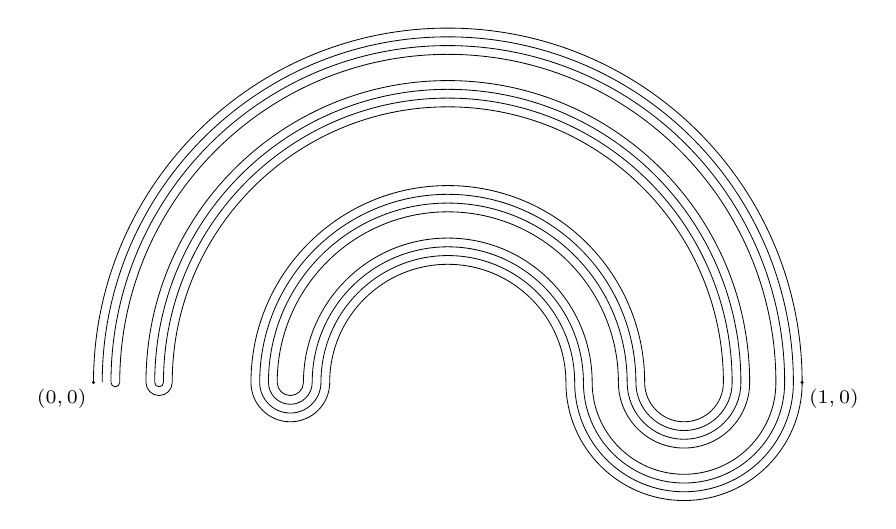
\begin{tikzpicture}[line width=0.3pt]
\draw (9,0) arc[start angle=0,end angle=180,radius=4.5];
\draw (8.88889,0) arc[start angle=0,end angle=180,radius=4.38889];
\draw (8.77778,0) arc[start angle=0,end angle=180,radius=4.27778];
\draw (8.66667,0) arc[start angle=0,end angle=180,radius=4.16667];
\draw (8.33333,0) arc[start angle=0,end angle=180,radius=3.83333];
\draw (8.22222,0) arc[start angle=0,end angle=180,radius=3.72222];
\draw (8.11111,0) arc[start angle=0,end angle=180,radius=3.61111];
\draw (8,0) arc[start angle=0,end angle=180,radius=3.5];
\draw (7,0) arc[start angle=0,end angle=180,radius=2.5];
\draw (6.88889,0) arc[start angle=0,end angle=180,radius=2.38889];
\draw (6.77778,0) arc[start angle=0,end angle=180,radius=2.27778];
\draw (6.66667,0) arc[start angle=0,end angle=180,radius=2.16667];
\draw (6.33333,0) arc[start angle=0,end angle=180,radius=1.83333];
\draw (6.22222,0) arc[start angle=0,end angle=180,radius=1.72222];
\draw (6.11111,0) arc[start angle=0,end angle=180,radius=1.61111];
\draw (6,0) arc[start angle=0,end angle=180,radius=1.5];
\draw (6,0) arc[start angle=180,end angle=360,radius=1.5];
\draw (6.11111,0) arc[start angle=180,end angle=360,radius=1.38889];
\draw (6.22222,0) arc[start angle=180,end angle=360,radius=1.27778];
\draw (6.33333,0) arc[start angle=180,end angle=360,radius=1.16667];
\draw (6.66667,0) arc[start angle=180,end angle=360,radius=0.83333];
\draw (6.77778,0) arc[start angle=180,end angle=360,radius=0.72222];
\draw (6.88889,0) arc[start angle=180,end angle=360,radius=0.61111];
\draw (7,0) arc[start angle=180,end angle=360,radius=0.5];
\draw (2,0) arc[start angle=180,end angle=360,radius=0.5];
\draw (2.11111,0) arc[start angle=180,end angle=360,radius=0.38889];
\draw (2.22222,0) arc[start angle=180,end angle=360,radius=0.27778];
\draw (2.33333,0) arc[start angle=180,end angle=360,radius=0.16667];
\draw (0.66667,0) arc[start angle=180,end angle=360,radius=0.16667];
\draw (0.77778,0) arc[start angle=180,end angle=360,radius=0.05556];
\draw (0.22222,0) arc[start angle=180,end angle=360,radius=0.05556];
\fill (0,0) circle[radius=0.6pt] node[below left=-1pt,font=\scriptsize] {$(0,0)$};
\fill (9,0) circle[radius=0.6pt] node[below right=-1pt,font=\scriptsize] {$(1,0)$};
\end{tikzpicture}
\caption{The Knaster bucket-handle continuum $K$, drawn at a finite stage. Let $C\subseteq[0,1]$ be the middle-thirds Cantor set. The continuum $K$ is the union of the upper semicircles centered at $(\frac12,0)$ that join points of $C$ symmetric about $\frac12$, together with, for each $n\ge1$, the lower semicircles centered at $(\frac{5}{2\cdot3^n},0)$ that join points of $C\cap[\frac{2}{3^n},\frac{1}{3^{n-1}}]$ symmetric about that center. The figure shows only the semicircles whose ends are endpoints of the $2^4$ intervals in the fourth stage of the construction of $C$.}
\label{fig:knaster}
\end{figure}

\begin{lemma}\label{lem:template}
There are points $\rho,r_\infty,r_1,r_2,\ldots\in K$ in pairwise distinct composants, with $r_m\to r_\infty$. There are also points $q,a_1,a_2,\ldots\in K$ in pairwise distinct composants such that $\{a_k:k\ge k_0\}$ is dense in $K$ for every $k_0\in\N$.
\end{lemma}

\begin{proof}
Choose $\rho$ and $r_\infty$ in distinct composants. Inductively choose $r_m\in N(r_\infty,1/m)$ in a composant avoiding $\rho,r_\infty,r_1,\dots,r_{m-1}$. This is possible since infinitely many dense composants remain (Fact~\ref{fact:indec}(b)). Next choose a sequence $V_1,V_2,\ldots$ of nonempty open sets such that every nonempty open set contains $V_k$ for infinitely many $k$, by repeating each member of a countable base infinitely often. Choose $q$, and then $a_k\in V_k$ in a composant avoiding $q,a_1,\dots,a_{k-1}$. Every index tail of this sequence is dense.
\end{proof}

The two families may share composants: only the first is used on blocks and only the second on spines. Put $T=\{\rho\}\cup\{r_m:m\in\N\}$. Its closure $T\cup\{r_\infty\}$ is countable and hence nowhere dense in $K$ by Fact~\ref{fact:indec}(d).

\subsection{The index tree}\label{subsec:tree}
Let $\Pc$ consist of symbols $B_\beta$, where $\beta$ is a finite, possibly empty, sequence of pairs in $\N\times\N$, and symbols $S_{\beta,m}$, where $m\in\N$. Call these symbols \emph{pieces}, with the former \emph{blocks} and the latter \emph{spines}. The same symbols index the abstract vertices of the tree and, after the realization in Section~\ref{subsec:realization}, the corresponding geometric pieces of $X$. Define
\[
\pa(S_{\beta,m})=B_\beta,\qquad \pa(B_{\beta^\frown(m,k)})=S_{\beta,m}.
\]
This is a rooted tree with root $B_\emptyset$. Write $M\preceq P$ when $M$ is a descendant of $P$, including $M=P$. Denote by $[P,R]$ the set of vertices on the unique tree path between $P$ and $R$. A set $F\subseteq\Pc$ is \emph{convex} if $[P,R]\subseteq F$ whenever $P,R\in F$.

The components of the tree with $M$ deleted are the descendant sets of its children and, when $M$ is non-root, the set of nondescendants of $M$. Distinct vertices $P,R\neq M$ lie in different such components exactly when $M\in[P,R]$. A simple path whose endpoints lie outside a descendant set never enters that set.

For a non-root piece $P$, let $t_P$ be the point of its parent's template where it is attached, and $o_P$ the point of its own template identified there. Set
\[
t_{S_{\beta,m}}=r_m,\qquad t_{B_{\beta^\frown(m,k)}}=a_k,\qquad
o_P=\begin{cases}\rho,&P\text{ is a non-root block},\\ q,&P\text{ is a spine}.\end{cases}
\]
Thus a non-root block meets its parent spine at the image of $\rho$ in its own template, and a spine meets its parent block at the image of $q$ in its own template. Set $o_{B_\emptyset}=(0,0)$ as a coordinate convention; it need not belong to $K$. The scales are
\[
\lambda_{B_\emptyset}=1,\qquad \lambda_{S_{\beta,m}}=2^{-(m+1)}\lambda_{B_\beta},\qquad \lambda_{B_{\beta^\frown(m,k)}}=2^{-(k+1)}\lambda_{S_{\beta,m}}.
\]
Every child has scale at most one quarter of its parent's scale, and each parent has finitely many children above any fixed positive scale. Put
\[
\Pc_N=\{P\in\Pc:\lambda_P\ge2^{-N}\}\qquad(N\ge0).
\]
For each non-root $P$, its own attaching point $o_P$ and the points $t_c$ for its children lie in pairwise distinct composants. Figure~\ref{fig:tree} shows the first levels of the tree schematically.

\begin{figure}[ht]
\centering
\begin{tikzpicture}[
  blk/.style={draw, rectangle, inner sep=2.5pt, font=\scriptsize},
  spn/.style={draw, ellipse, inner sep=1.5pt, font=\scriptsize},
  lab/.style={font=\tiny, fill=white, inner sep=1pt}]
\node[blk] (R) at (0,0) {$B_\emptyset$};
\node[spn] (S1) at (-4,-1.7) {$S_{\emptyset,1}$};
\node[spn] (S2) at (0.8,-1.7) {$S_{\emptyset,2}$};
\node[spn] (S3) at (4.2,-1.7) {$S_{\emptyset,3}$};
\node at (5.8,-1.7) {$\cdots$};
\draw (R) -- node[lab] {$r_1$} (S1);
\draw (R) -- node[lab] {$r_2$} (S2);
\draw (R) -- node[lab] {$r_3$} (S3);
\node[blk] (B11) at (-6.3,-3.4) {$B_{(1,1)}$};
\node[blk] (B12) at (-4.3,-3.4) {$B_{(1,2)}$};
\node[blk] (B13) at (-2.4,-3.4) {$B_{(1,3)}$};
\node at (-1.1,-3.4) {$\cdots$};
\draw (S1) -- node[lab] {$a_1$} (B11);
\draw (S1) -- node[lab] {$a_2$} (B12);
\draw (S1) -- node[lab] {$a_3$} (B13);
\node[blk] (B21) at (0.3,-3.4) {$B_{(2,1)}$};
\node[blk] (B22) at (2.2,-3.4) {$B_{(2,2)}$};
\node at (3.4,-3.4) {$\cdots$};
\draw (S2) -- node[lab] {$a_1$} (B21);
\draw (S2) -- node[lab] {$a_2$} (B22);
\node[spn] (T1) at (-7.2,-5.1) {$S_{(1,1),1}$};
\node[spn] (T2) at (-5.1,-5.1) {$S_{(1,1),2}$};
\node at (-3.7,-5.1) {$\cdots$};
\draw (B11) -- node[lab] {$r_1$} (T1);
\draw (B11) -- node[lab] {$r_2$} (T2);
\end{tikzpicture}
\caption{Schematic picture of the first levels of the index tree $\Pc$. Rectangles are blocks and ellipses are spines. The label on an edge is the template point $t_c$ of the parent at which the child $c$ is attached: $r_m$ for the spine $S_{\beta,m}$ and $a_k$ for the block $B_{\beta^\frown(m,k)}$. Every block has infinitely many child spines and every spine has infinitely many child blocks, as indicated by the dots. The picture is only schematic: in the construction the pieces are scaled copies of $K$ placed in pairwise orthogonal planes of $\ell^2$, not in the plane of the drawing.}
\label{fig:tree}
\end{figure}

\subsection{Realization in Hilbert space}\label{subsec:realization}
We now realize the abstract tree geometrically in $\ell^2$. Each piece $P$ is represented by a copy of the same continuum $K$, scaled by the factor $\lambda_P$ and attached to its parent at the image of the prescribed template point. Every piece receives its own two-dimensional coordinate plane, orthogonal to the planes of all other pieces, so that distinct pieces can be separated by orthogonal projections, while the rapidly decreasing scales keep all descendants of a piece within a small ball around the point where that piece is attached. Lemmas~\ref{lem:coordinates} and~\ref{lem:geometry} establish the separation and compactness properties needed later.

Concretely, fix an orthonormal family $\{e_P,f_P:P\in\Pc\}$ in $\ell^2$. Let $E_P=\operatorname{span}\{e_P,f_P\}$, let $J_P\colon\R^2\to E_P$ be the isometry $J_P(x,y)=xe_P+yf_P$, and let $\pi_P$ be orthogonal projection onto $E_P$. Set $p_{B_\emptyset}=0$ and define recursively
\[
\varphi_P(z)=p_P+\lambda_PJ_P(z-o_P),\qquad p_P=\varphi_{\pa(P)}(t_P)\quad(P\neq B_\emptyset).
\]
Thus $\varphi_{B_\emptyset}=J_{B_\emptyset}|_K$. Identify each piece $P$ with $\varphi_P(K)$. For a non-root piece, $\varphi_P(o_P)=p_P\in P\cap\pa(P)$. The root point $p_{B_\emptyset}$ is not an attaching point and is not required to lie in $B_\emptyset$.

Define closed sets
\[
Y_P=\operatorname{cl}_{\ell^2}\bigcup_{M\preceq P}M,\qquad X=Y_{B_\emptyset},\qquad Z_P=\operatorname{cl}_{\ell^2}\bigcup_{M\not\preceq P}M\quad(P\neq B_\emptyset).
\]
All closures of subsets of $X$ may be taken either in $X$ or in $\ell^2$, since $X$ is closed. We use the norm metric.

\begin{lemma}[Coordinates]\label{lem:coordinates}
Let $B_\emptyset=P_0,P_1,\ldots,P_n=M$ be the root path of $M$. For $z\in K$ and $x=\varphi_M(z)$, put $w_i=t_{P_{i+1}}$ for $i<n$ and $w_n=z$. Then
\[
\pi_{P_i}(x)=\lambda_{P_i}J_{P_i}(w_i-o_{P_i})\quad(0\le i\le n),\qquad \pi_R(x)=0\quad\bigl(R\notin\{P_0,\ldots,P_n\}\bigr).
\]
\end{lemma}

\begin{proof}
Since $p_{P_{i+1}}=\varphi_{P_i}(t_{P_{i+1}})=p_{P_i}+\lambda_{P_i}J_{P_i}(t_{P_{i+1}}-o_{P_i})$ for $i<n$, and $p_{B_\emptyset}=0$, $o_{B_\emptyset}=(0,0)$, unfolding the recursion along the root path gives
\[
x=p_M+\lambda_MJ_M(z-o_M)=\sum_{i=0}^{n}\lambda_{P_i}J_{P_i}(w_i-o_{P_i}).
\]
The $i$-th summand lies in $E_{P_i}$, and the planes $E_P$, $P\in\Pc$, are pairwise orthogonal. Applying $\pi_{P_i}$, or $\pi_R$ for $R$ off the root path, gives the assertion.
\end{proof}

The following lemma collects the geometric properties of the realization. Parts (a)--(b) control the sizes of subtrees; parts (c)--(g) describe how subtrees intersect and how they are separated; part (h) shows that $X$ is a continuum.

\begin{lemma}[Geometry of $X$]\label{lem:geometry}
\begin{enumerate}[label=\textup{(\alph*)}]
\item Every $\Pc_N$ is finite, contains the root, and contains the parent of each of its non-root members.
\item If $P\neq B_\emptyset$ and $x\in Y_P$, then $\|x-p_P\|\le\frac43\lambda_P$. In particular, $\diam Y_P\le3\lambda_P$.
\item For every piece $P$, one has $Y_P=P\cup\bigcup_cY_c$, where $c$ ranges over the children of $P$.
\item For every $P$, including the root, $\pi_P$ is constant on each child subtree $Y_c$:
\[
\pi_P(Y_c)=\{\lambda_PJ_P(t_c-o_P)\}.
\]
\item If $P\neq B_\emptyset$, then $\pi_P$ vanishes on $Z_P$, and for $x\in Y_P$ it vanishes if and only if $x=p_P$.
\item Distinct children $c,c'$ of $P$ satisfy $Y_c\cap Y_{c'}=\emptyset$, and $Y_c\cap P=\{p_c\}$.
\item If $P\neq B_\emptyset$, then $X=Y_P\cup Z_P$ and $Y_P\cap Z_P=\{p_P\}$. Thus $Y_P\setminus\{p_P\}=X\setminus Z_P$ and $Z_P\setminus\{p_P\}=X\setminus Y_P$ are open in $X$.
\item The space $X$ is a continuum. Along any infinite branch $B_\emptyset=P_0,P_1,\ldots$,
\[
\diam Y_{P_n}\le3\lambda_{P_n}\le3\cdot4^{-(n-1)}\lambda_{P_1}\qquad(n\ge1),
\]
and $\bigcap_nY_{P_n}$ is a singleton. Every point of $X$ either belongs to a piece or is the point of such an intersection.
\end{enumerate}
\end{lemma}

\begin{proof}
\emph{Tree and scale estimates.} (a) Every step multiplies the scale by $2^{-(j+1)}$ with $j\ge1$. The inequality $\lambda_P\ge2^{-N}$ therefore bounds depth by $N/2$ and bounds each index in the name of $P$. There are finitely many such names, and scales decrease along paths away from the root.

(b) Suppose $x\in M\preceq P$, and write $P=M_0,M_1,\ldots,M_j=M$. Then
\[
x-p_P=\sum_{i<j}(p_{M_{i+1}}-p_{M_i})+(x-p_M).
\]
All these pieces are non-root. Each displacement in $M_i$ has norm at most $\lambda_{M_i}\diam K=\lambda_{M_i}$, and $\|x-p_M\|\le\lambda_M$. Thus
\[
\|x-p_P\|\le\lambda_P\sum_{i\ge0}4^{-i}=\tfrac43\lambda_P.
\]
The bound passes to the closure; the diameter is at most $\frac83\lambda_P\le3\lambda_P$.

\emph{Subtree decomposition and separation.} (c) Only the inclusion from left to right needs proof. Choose $x_n\to y\in Y_P$, with $x_n$ in descendant pieces. If a subsequence lies in $P$ or in a fixed $Y_c$, closedness gives the conclusion. Otherwise pass to a subsequence lying in pairwise distinct child subtrees $Y_{c_n}$. Then $\lambda_{c_n}\to0$, so (b) gives $\|x_n-p_{c_n}\|\to0$. Since $p_{c_n}\in P$ and $P$ is compact, $y\in P$. This uses no compactness assumption on $X$.

(d) The root path of every descendant of $c$ passes through $P$ and then $c$. Lemma~\ref{lem:coordinates} therefore gives the specified coordinate on the descendant union, and continuity extends it to $Y_c$.

(e) For a nondescendant $M$ of $P$, the root path omits $P$, so the coordinate vanishes on $M$ and hence on $Z_P$. On $P$ it vanishes exactly at $\varphi_P(o_P)=p_P$. On $Y_c$ its constant value from (d) is nonzero, because $t_c$ and $o_P$ lie in distinct composants. Part (c) exhausts $Y_P$.

(f) Apply (e) to the non-root child $c$. Its coordinate vanishes on $Y_{c'}\cup P\subseteq Z_c$ and vanishes on $Y_c$ only at $p_c$. Thus $Y_c\cap Y_{c'}\subseteq\{p_c\}$, and symmetrically it is contained in $\{p_{c'}\}$. Since $t_c\neq t_{c'}$ and $\varphi_P$ is injective, these points differ. The same argument gives $Y_c\cap P=\{p_c\}$.

(g) Every piece is either a descendant of $P$ or a nondescendant, so $X=Y_P\cup Z_P$. Part (e) gives $Y_P\cap Z_P\subseteq\{p_P\}$, and $p_P\in\pa(P)\subseteq Z_P$. The open-set identities follow by taking complements of closed sets.

\emph{Compactness and connectedness.} (h) For a piece outside $\Pc_N$, let $P$ be the first vertex outside $\Pc_N$ on its root path. Its parent belongs to $\Pc_N$. Part (b) puts every point of that piece within $\frac43\lambda_P<\frac43\cdot2^{-N}$ of $p_P\in\bigcup\Pc_N$. The finite union $\bigcup\Pc_N$ is compact, so these estimates prove total boundedness of the union of all pieces. Its closure in the complete space $\ell^2$ is compact. The unions $\bigcup\Pc_N$ are connected, since their vertices are joined to the root by paths of incident pieces; they increase and exhaust the piece union. Hence $X$ is connected.

Along an infinite branch, the displayed diameter bound follows from (b) and the scale recursion. The nonempty compact sets $Y_{P_n}$ decrease and their diameters tend to zero, so their intersection is a singleton. If $y$ lies in no piece, part (c) successively places it in a child subtree at each level, giving the required infinite branch.
\end{proof}

\begin{remark}\label{rem:closures}
The intersection identities in Lemma~\ref{lem:geometry}(e)--(g) show that taking closures introduces no additional contacts between a subtree and its complement. This includes limit points of infinitely many small subtrees. Separation follows from the coordinates of the relevant child, together with the distinct attachment coordinates on its parent.
\end{remark}

For a piece $M$, let $\At(M)$ consist of its child attaching points $p_c$, and additionally $p_M$ when $M$ is non-root. Any other piece meets $M$, if at all, only in $\At(M)$: descendant pieces lie in a child subtree, and nondescendants, when present, lie in $Z_M$.

Figure~\ref{fig:block-spine} illustrates the next lemma: the attaching points on a block form a small set, while the child attachments on a spine are dense.

\begin{lemma}[Interiors]\label{lem:interiors}
\begin{enumerate}[label=\textup{(\alph*)}]
\item For every block $B$, $\intX B$ is dense in $B$ and disjoint from $\At(B)$. It meets no other piece.
\item Every spine has empty interior in $X$.
\item The set $U=\bigcup\{\intX B: B\text{ is a block}\}$ is open and dense in $X$.
\end{enumerate}
\end{lemma}

\begin{proof}
(a) Put $D=\clX\At(B)$. The child attaching points of $B=B_\beta$ are $p_{S_{\beta,m}}=\varphi_B(t_{S_{\beta,m}})=\varphi_B(r_m)$. When $B$ is non-root, its own attaching point is $p_B=\varphi_B(o_B)=\varphi_B(\rho)$. Hence $\At(B)\subseteq\varphi_B(T)$, and $D$ is contained in the countable compact set $\varphi_B(\operatorname{cl}_KT)$. Thus $B\setminus D$ is dense in $B$ by Fact~\ref{fact:indec}(d). Fix $x\in B\setminus D$ and $\delta=d(x,D)>0$. There are only finitely many children $c$ with $\frac43\lambda_c\ge\delta/2$; call this finite set $\Ec$. For these children, $x\notin Y_c$ and hence $d(x,Y_c)>0$. For the others,
\[
d(x,Y_c)\ge d(x,p_c)-\tfrac43\lambda_c>\delta/2.
\]
When $B$ is non-root, also $d(x,Z_B)>0$. Choose $\eta>0$ smaller than $\delta/2$, all $d(x,Y_c)$ for $c\in\Ec$, and, only in the non-root case, $d(x,Z_B)$. The decomposition of Lemma~\ref{lem:geometry}(c),(g) gives $N(x,\eta)\subseteq B$. For the root the parent-side term is simply absent.

Conversely, each $w\in\At(B)$ is the unique intersection of $B$ with an incident nondegenerate piece. Such a piece has points different from $w$ arbitrarily close to $w$, all outside $B$. Thus $w\notin\intX B$. Since other pieces meet $B$ only at its attachments, the last assertion follows.

(b) Fix $x\in S$ and $\eta>0$. Choose $k_0$ so that $\frac43\cdot2^{-(k_0+1)}\lambda_S<\eta/2$. Tail density gives $k\ge k_0$ with $\|\varphi_S(a_k)-x\|<\eta/2$. The child block attached there lies in $N(x,\eta)$ by Lemma~\ref{lem:geometry}(b) and contains points outside $S$. Thus $x$ is not interior to $S$.

(c) Openness is immediate. Block points lie in $\clX U$ by (a). The argument in (b) approximates every spine point by child-block points, hence by points of $U$. Finally, a branch limit is approximated by points in the even-level blocks on its branch, since the subtree diameters tend to zero. Lemma~\ref{lem:geometry}(h) exhausts $X$.
\end{proof}

\begin{figure}[ht]
\centering
% Schematic: left, a block with child spines at points converging to phi_B(r_infty);
% right, a spine with child blocks at a dense set of points.
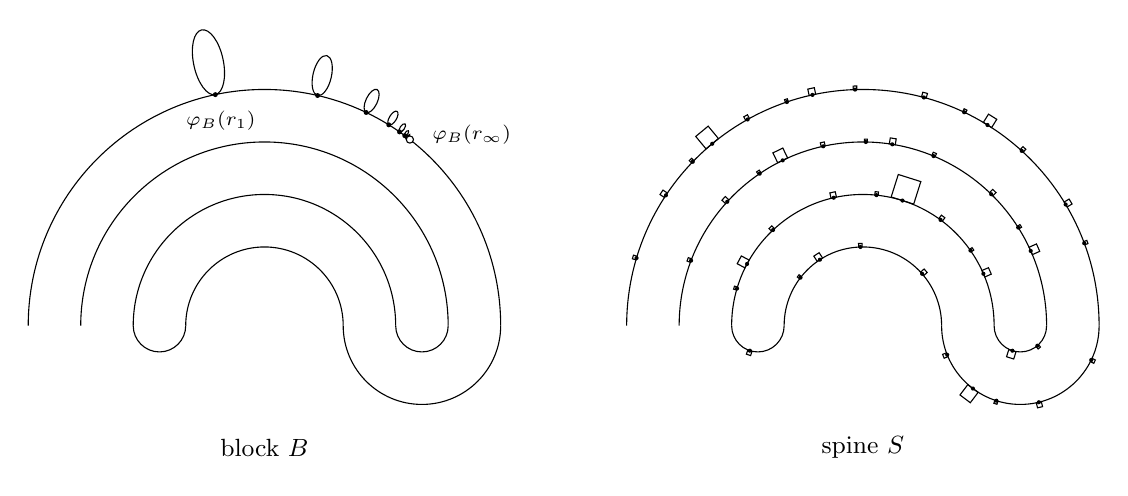
\begin{tikzpicture}[line width=0.4pt]
\draw (6,0) arc[start angle=0,end angle=180,radius=3];
\draw (5.33333,0) arc[start angle=0,end angle=180,radius=2.33333];
\draw (4.66667,0) arc[start angle=0,end angle=180,radius=1.66667];
\draw (4,0) arc[start angle=0,end angle=180,radius=1];
\draw (4,0) arc[start angle=180,end angle=360,radius=1];
\draw (4.66667,0) arc[start angle=180,end angle=360,radius=0.33333];
\draw (1.33333,0) arc[start angle=180,end angle=360,radius=0.33333];
\draw[rotate around={102:(2.28894,3.34526)}] (2.28894,3.34526) ellipse[x radius=0.42,y radius=0.189];
\fill (2.37626,2.93444) circle[radius=0.9pt];
\draw[rotate around={77:(3.73343,3.17684)}] (3.73343,3.17684) ellipse[x radius=0.2604,y radius=0.11718];
\fill (3.67485,2.92311) circle[radius=0.9pt];
\draw[rotate around={64.5:(4.36104,2.85348)}] (4.36104,2.85348) ellipse[x radius=0.16145,y radius=0.07265];
\fill (4.29153,2.70776) circle[radius=0.9pt];
\draw[rotate around={58.25:(4.63131,2.63618)}] (4.63131,2.63618) ellipse[x radius=0.1001,y radius=0.04504];
\fill (4.57864,2.55106) circle[radius=0.9pt];
\draw[rotate around={55.125:(4.75085,2.51212)}] (4.75085,2.51212) ellipse[x radius=0.06206,y radius=0.02793];
\fill (4.71536,2.4612) circle[radius=0.9pt];
\draw[rotate around={53.5625:(4.80469,2.44447)}] (4.80469,2.44447) ellipse[x radius=0.03848,y radius=0.01731];
\fill (4.78184,2.41352) circle[radius=0.9pt];
\draw[rotate around={52.78125:(4.82901,2.40799)}] (4.82901,2.40799) ellipse[x radius=0.02386,y radius=0.01074];
\fill (4.81458,2.389) circle[radius=0.9pt];
\filldraw[fill=white] (4.84698,2.36403) circle[radius=1.3pt];
\node[font=\scriptsize,anchor=west] at (5.00698,2.42403) {$\varphi_B(r_\infty)$};
\node[font=\scriptsize] at (2.44695,2.60187) {$\varphi_B(r_1)$};
\node[font=\small] at (3,-1.55) {block $B$};
\draw (13.6,0) arc[start angle=0,end angle=180,radius=3];
\draw (12.93333,0) arc[start angle=0,end angle=180,radius=2.33333];
\draw (12.26667,0) arc[start angle=0,end angle=180,radius=1.66667];
\draw (11.6,0) arc[start angle=0,end angle=180,radius=1];
\draw (11.6,0) arc[start angle=180,end angle=360,radius=1];
\draw (12.26667,0) arc[start angle=180,end angle=360,radius=0.33333];
\draw (8.93333,0) arc[start angle=180,end angle=360,radius=0.33333];
\draw (11.24535,1.54396)--(11.33576,1.83001)--(11.04971,1.92043)--(10.9593,1.63438)--cycle;
\fill (11.10232,1.58917) circle[radius=0.75pt];
\draw (8.7658,2.37618)--(8.63514,2.53401)--(8.4773,2.40334)--(8.60797,2.24551)--cycle;
\fill (8.68689,2.31084) circle[radius=0.75pt];
\draw (11.9322,-0.74884)--(11.83345,-0.87971)--(11.96431,-0.97846)--(12.06307,-0.8476)--cycle;
\fill (11.99763,-0.79822) circle[radius=0.75pt];
\draw (9.64441,2.12983)--(9.58331,2.25575)--(9.4574,2.19465)--(9.51849,2.06874)--cycle;
\fill (9.58145,2.09928) circle[radius=0.75pt];
\draw (12.23509,2.51601)--(12.30039,2.62118)--(12.19522,2.68648)--(12.12992,2.58131)--cycle;
\fill (12.1825,2.54866) circle[radius=0.75pt];
\draw (9.1554,0.83308)--(9.05657,0.88574)--(9.00391,0.78691)--(9.10274,0.73426)--cycle;
\fill (9.12907,0.78367) circle[radius=0.75pt];
\draw (12.7524,0.90237)--(12.84638,0.94422)--(12.80452,1.0382)--(12.71054,0.99634)--cycle;
\fill (12.73147,0.94935) circle[radius=0.75pt];
\draw (12.45339,-0.30315)--(12.42441,-0.39424)--(12.5155,-0.42323)--(12.54448,-0.33213)--cycle;
\fill (12.49894,-0.31764) circle[radius=0.75pt];
\draw (12.14815,0.61888)--(12.23042,0.65436)--(12.19494,0.73663)--(12.11267,0.70115)--cycle;
\fill (12.13041,0.66001) circle[radius=0.75pt];
\draw (10.00086,2.93987)--(9.98281,3.02247)--(9.9002,3.00442)--(9.91825,2.92182)--cycle;
\fill (9.95955,2.93084) circle[radius=0.75pt];
\draw (10.08784,0.85983)--(10.04406,0.92706)--(9.97683,0.88327)--(10.02061,0.81604)--cycle;
\fill (10.05423,0.83793) circle[radius=0.75pt];
\draw (11.01123,2.29713)--(11.02347,2.37263)--(10.94798,2.38487)--(10.93573,2.30937)--cycle;
\fill (10.97348,2.30325) circle[radius=0.75pt];
\draw (13.19381,1.50781)--(13.25663,1.54537)--(13.21908,1.60819)--(13.15626,1.57064)--cycle;
\fill (13.17503,1.53922) circle[radius=0.75pt];
\draw (10.26437,1.6329)--(10.24877,1.70141)--(10.18026,1.68582)--(10.19585,1.61731)--cycle;
\fill (10.23011,1.6251) circle[radius=0.75pt];
\draw (8.11731,1.68446)--(8.06091,1.72181)--(8.02356,1.66541)--(8.07997,1.62806)--cycle;
\fill (8.09864,1.65626) circle[radius=0.75pt];
\draw (12.80285,-0.97975)--(12.81816,-1.04322)--(12.88163,-1.02791)--(12.86632,-0.96444)--cycle;
\fill (12.83458,-0.9721) circle[radius=0.75pt];
\draw (8.89905,1.59756)--(8.85243,1.64016)--(8.80983,1.59355)--(8.85644,1.55095)--cycle;
\fill (8.87774,1.57425) circle[radius=0.75pt];
\draw (11.40439,2.89031)--(11.4202,2.94943)--(11.36108,2.96523)--(11.34527,2.90611)--cycle;
\fill (11.37483,2.89821) circle[radius=0.75pt];
\draw (11.37204,0.63626)--(11.41674,0.67539)--(11.37762,0.72009)--(11.33292,0.68096)--cycle;
\fill (11.35248,0.65861) circle[radius=0.75pt];
\draw (12.2504,1.64969)--(12.29073,1.69102)--(12.24941,1.73135)--(12.20907,1.69002)--cycle;
\fill (12.22973,1.66985) circle[radius=0.75pt];
\draw (9.13784,-0.30872)--(9.12063,-0.36224)--(9.17415,-0.37945)--(9.19136,-0.32593)--cycle;
\fill (9.1646,-0.31732) circle[radius=0.75pt];
\draw (11.60894,1.32687)--(11.64139,1.37103)--(11.59722,1.40348)--(11.56478,1.35931)--cycle;
\fill (11.58686,1.34309) circle[radius=0.75pt];
\draw (9.15998,2.63193)--(9.13389,2.67861)--(9.08721,2.65253)--(9.11329,2.60584)--cycle;
\fill (9.13663,2.61889) circle[radius=0.75pt];
\draw (11.66111,-0.34521)--(11.61257,-0.36452)--(11.63187,-0.41306)--(11.68041,-0.39376)--cycle;
\fill (11.67076,-0.36949) circle[radius=0.75pt];
\draw (10.12079,2.28374)--(10.10975,2.33361)--(10.05988,2.32257)--(10.07091,2.2727)--cycle;
\fill (10.09585,2.27822) circle[radius=0.75pt];
\draw (12.63608,2.20341)--(12.66969,2.24041)--(12.6327,2.27403)--(12.59908,2.23703)--cycle;
\fill (12.61758,2.22022) circle[radius=0.75pt];
\draw (9.47722,1.23197)--(9.44371,1.26767)--(9.40801,1.23416)--(9.44152,1.19846)--cycle;
\fill (9.45937,1.21521) circle[radius=0.75pt];
\draw (7.73253,0.88214)--(7.68654,0.89588)--(7.6728,0.8499)--(7.71878,0.83615)--cycle;
\fill (7.72565,0.85914) circle[radius=0.75pt];
\draw (13.48986,-0.45683)--(13.53224,-0.47734)--(13.55275,-0.43497)--(13.51037,-0.41446)--cycle;
\fill (13.50012,-0.43565) circle[radius=0.75pt];
\draw (8.42607,0.84793)--(8.38285,0.8643)--(8.36649,0.82108)--(8.4097,0.80472)--cycle;
\fill (8.41788,0.82633) circle[radius=0.75pt];
\draw (10.52316,2.9991)--(10.52166,3.04446)--(10.4763,3.04295)--(10.47781,2.9976)--cycle;
\fill (10.50049,2.99835) circle[radius=0.75pt];
\draw (10.59086,1.00021)--(10.58946,1.04478)--(10.54489,1.04338)--(10.54629,0.99881)--cycle;
\fill (10.56858,0.99951) circle[radius=0.75pt];
\draw (11.51748,2.14549)--(11.53435,2.18597)--(11.49387,2.20283)--(11.47701,2.16236)--cycle;
\fill (11.49725,2.15392) circle[radius=0.75pt];
\draw (13.41859,1.02763)--(13.459,1.0427)--(13.44394,1.08312)--(13.40352,1.06805)--cycle;
\fill (13.41105,1.04784) circle[radius=0.75pt];
\draw (10.79368,1.65551)--(10.79808,1.69773)--(10.75586,1.70213)--(10.75146,1.65991)--cycle;
\fill (10.77257,1.65771) circle[radius=0.75pt];
\draw (8.45415,2.09661)--(8.42405,2.12561)--(8.39505,2.09551)--(8.42515,2.06651)--cycle;
\fill (8.43965,2.08156) circle[radius=0.75pt];
\draw (12.2762,-0.94635)--(12.26367,-0.98557)--(12.3029,-0.99809)--(12.31542,-0.95887)--cycle;
\fill (12.29581,-0.95261) circle[radius=0.75pt];
\draw (9.30639,1.94201)--(9.2836,1.97559)--(9.25003,1.9528)--(9.27282,1.91923)--cycle;
\fill (9.2896,1.93062) circle[radius=0.75pt];
\draw (11.90456,2.70158)--(11.92171,2.73771)--(11.88558,2.75486)--(11.86843,2.71873)--cycle;
\fill (11.88649,2.71015) circle[radius=0.75pt];
\draw (9.00713,0.49086)--(8.9693,0.50203)--(8.95813,0.4642)--(8.99597,0.45303)--cycle;
\fill (9.00155,0.47195) circle[radius=0.75pt];
\draw (12.58284,1.23011)--(12.61573,1.2509)--(12.59494,1.2838)--(12.56205,1.26301)--cycle;
\fill (12.57244,1.24656) circle[radius=0.75pt];
\draw (12.80114,-0.2665)--(12.826,-0.29577)--(12.85527,-0.27091)--(12.83041,-0.24164)--cycle;
\fill (12.81578,-0.25407) circle[radius=0.75pt];
\draw (11.97732,0.93868)--(12.0084,0.96038)--(11.9867,0.99146)--(11.95562,0.96976)--cycle;
\fill (11.96647,0.95422) circle[radius=0.75pt];
\draw (9.65242,2.84648)--(9.64038,2.88192)--(9.60494,2.86987)--(9.61698,2.83444)--cycle;
\fill (9.6347,2.84046) circle[radius=0.75pt];
\draw (9.81891,0.62469)--(9.78961,0.64724)--(9.76706,0.61795)--(9.79636,0.5954)--cycle;
\fill (9.80763,0.61004) circle[radius=0.75pt];
\draw (10.65598,2.33273)--(10.65657,2.36925)--(10.62005,2.36985)--(10.61946,2.33332)--cycle;
\fill (10.63772,2.33303) circle[radius=0.75pt];
\node[font=\small] at (10.6,-1.55) {spine $S$};
\end{tikzpicture}
\caption{Schematic comparison of a block and a spine. Both are scaled copies of $K$, drawn here at a coarse stage of the construction in Figure~\ref{fig:knaster}. Left: the child spines of a block $B$ (small ellipses) are attached at the points $\varphi_B(r_m)$, which converge to $\varphi_B(r_\infty)$ (open circle). Together with the attaching point $p_B=\varphi_B(\rho)$ of $B$ itself (when $B$ is not the root), these points lie in the countable closed set $\varphi_B(T\cup\{r_\infty\})$, which is nowhere dense in $B$; together with the subtree estimates, this gives density of $\intX B$ in $B$ (see Lemma~\ref{lem:interiors}(a)). Right: the child blocks of a spine $S$ (small squares) are attached at the points $\varphi_S(a_k)$, which are dense in $S$. Every point of $S$ is therefore a limit of points of $X\setminus S$, and $S$ has empty interior in $X$ (Lemma~\ref{lem:interiors}(b)). The children shrink, and only finitely many of them exceed any given size; in the construction they lie in planes of $\ell^2$ orthogonal to the plane of their parent. Blocks supply the interior from which regular subcontinua are built (Lemma~\ref{lem:blocks-generate}), and spines impose the density condition~(c) of Theorem~\ref{thm:description}. Remark~\ref{rem:spines} shows that spines are needed, Remark~\ref{rem:leaf} that every block must carry spines, and Remark~\ref{rem:blocks} records the role of blocks.}
\label{fig:block-spine}
\end{figure}

\section{\texorpdfstring{The regular subcontinua of $X$}{The regular subcontinua of X}}\label{sec:regular}

\begin{definition}\label{def:branches}
For $M\in\Pc$, the \emph{branches} at $M$ are $W_c=Y_c\setminus\{p_c\}$ for the children $c$ of $M$, with attaching points $p_c$, and, only when $M\neq B_\emptyset$, the set $W_-=Z_M\setminus\{p_M\}$ with attaching point $p_M$.
\end{definition}

\begin{lemma}[Branches]\label{lem:branches}
Let $M\in\Pc$.
\begin{enumerate}[label=\textup{(\alph*)}]
\item The branches at $M$ are open, pairwise disjoint, and disjoint from $M$, and together with $M$ they cover $X$.
\item If $W$ is a branch with attaching point $w$, then $W\cup\{w\}$ is closed and meets $M$ exactly at $w$.
\item The attaching points of distinct branches correspond under $\varphi_M$ to points in distinct composants of $K$.
\item Every piece $R\neq M$ lies in $W\cup\{w\}$ for exactly one branch $W$, and meets $W$. Two pieces $R,R'\neq M$ correspond to different branches exactly when $M\in[R,R']$.
\end{enumerate}
\end{lemma}

\begin{proof}
Every statement involving $W_-$, $Z_M$, or the parent attaching point $p_M$ in this proof is restricted to non-root $M$.

(a) Each $W_c=X\setminus Z_c$ is open, since children are non-root. Distinct child branches are disjoint by Lemma~\ref{lem:geometry}(f), and each is disjoint from $M$. At the root, Lemma~\ref{lem:geometry}(c) gives the entire decomposition. At a non-root $M$, the additional branch $W_-=X\setminus Y_M$ is open and disjoint from $M$ and all child branches. Parts (c) and (g) of that lemma give the full decomposition, since all the omitted attaching points belong to $M$.

(b) The relevant one-point enlargements are $Y_c$, and, in the non-root case, $Z_M$. The assertion follows from Lemma~\ref{lem:geometry}(f),(g).

(c) At the root, the attaching points are $\varphi_M(r_m)$, which lie in distinct composants by Lemma~\ref{lem:template}. At a non-root piece the template points are its child attachment points $t_c$ and its own attaching point $o_M$, again in distinct composants by construction.

(d) If $R\preceq c$ for a child $c$, then $R\subseteq Y_c$; otherwise, at a non-root $M$, one has $R\subseteq Z_M$. A nondegenerate piece cannot be contained in the single attaching point, so it meets the corresponding branch. The closed one-point enlargements of two distinct branches are disjoint: the open branches are disjoint, meet no point of $M$, and have distinct attaching points. This proves uniqueness. The last assertion follows from the components of the abstract tree with $M$ deleted.
\end{proof}

\begin{lemma}[Retractions and crossing]\label{lem:retraction}
For $M\in\Pc$, define $r_M\colon X\to\ell^2$ by $r_M(x)=p_M+\pi_M(x)$, with $p_{B_\emptyset}=0$.
\begin{enumerate}[label=\textup{(\roman*)}]
\item The map $r_M$ takes values in $M$ and is a $1$-Lipschitz retraction of $X$ onto $M$. For each branch $W$ at $M$ with attaching point $w$, it maps $W\cup\{w\}$ to $w$.
\item For $A\in C(X)$, the set $r_M(A)$ is a subcontinuum of $M$ and
\[
r_M(A)=(A\cap M)\cup\{w: W\text{ is a branch at }M,\ A\cap W\neq\emptyset\}\subseteq(A\cap M)\cup\At(M).
\]
\item If $A\in C(X)$ meets $W$ but is not contained in $W$, then $w\in A$. If $A$ is not contained in a single branch at $M$, then $r_M(A)\subseteq A$.
\item If $A\in C(X)$ meets two distinct branches at $M$, then $M\subseteq A$.
\end{enumerate}
\end{lemma}

\begin{proof}
(i) Orthogonal projection gives $\|r_M(x)-r_M(y)\|=\|\pi_M(x-y)\|\le\|x-y\|$. On $M$, Lemma~\ref{lem:coordinates} gives $r_M(\varphi_M(z))=\varphi_M(z)$. On $Y_c$, Lemma~\ref{lem:geometry}(d) gives
\[
r_M(x)=p_M+\lambda_MJ_M(t_c-o_M)=p_c.
\]
For a non-root $M$, part (e) of that lemma gives $r_M(x)=p_M$ on $Z_M$. These cases cover $X$ by Lemma~\ref{lem:branches}, and in each case the value lies in $M$. From now on we regard $r_M$ as a map $X\to M$.

(ii) This follows from (i) and the branch decomposition, since the continuous image of a continuum is a continuum.

(iii) If $w\notin A$, the disjoint open sets $W$ and $X\setminus(W\cup\{w\})$ cover $A$. The assumptions force $A$ to meet both, contradicting connectedness. If $A$ is not contained in any single branch, apply this conclusion to every branch it meets and use (ii).

(iv) By (iii), $r_M(A)\subseteq A$. This subcontinuum of $M$ contains the attaching points of two distinct branches, which lie in distinct composants by Lemma~\ref{lem:branches}(c). Fact~\ref{fact:indec}(c) forces $r_M(A)=M$.
\end{proof}

\begin{lemma}[Pieces are atoms]\label{lem:atoms}
If $A\in C(X)$ and $P$ is a piece with $\intX A\cap P\neq\emptyset$, then $P\subseteq A$.
\end{lemma}

\begin{proof}
The set $\intX A\cap P$ is a nonempty relatively open subset of $P$ contained in the subcontinuum $r_P(A)$. Fact~\ref{fact:indec}(a) gives $r_P(A)=P$. Lemma~\ref{lem:retraction}(ii) then gives $P\setminus\At(P)\subseteq A$. Since $\At(P)$ is countable, its complement is dense in $P$ by Fact~\ref{fact:indec}(d), and closedness yields $P\subseteq A$.
\end{proof}

The lemma holds for every piece, but it is used below only for blocks. For a block $B$ and $A\in\D(X)$, its hypothesis holds as soon as $A$ meets $\intX B$, by regularity of $A$.

\begin{lemma}[Regularity comes from blocks]\label{lem:blocks-generate}
Every block is regular closed in $X$. For every $A\in\D(X)$,
\[
A=\clX\bigcup\{B: B\text{ is a block and }B\subseteq A\}.
\]
Conversely, the closure of the union of any nonempty family of blocks is regular closed in $X$.
\end{lemma}

\begin{proof}
Blocks are regular closed by Lemma~\ref{lem:interiors}(a). The dense open set $U$ from part (c) of that lemma meets $\intX A$ densely in $\intX A$. Every such point lies in the interior of a block meeting $\intX A$, and Lemma~\ref{lem:atoms} puts that entire block in $A$. Thus regularity of $A$ gives the displayed equality. The converse is Lemma~\ref{lem:regular-closed}.
\end{proof}

Lemma~\ref{lem:blocks-generate} shows that a regular subcontinuum is determined by the blocks it contains. The next theorem characterizes exactly which collections of pieces arise in this way, and its proof shows where each condition comes from. Convexity is forced by crossing indecomposable pieces: a subcontinuum that meets two branches at a piece $M$ must contain all of $M$ (Lemma~\ref{lem:retraction}(iv)), because attaching points in distinct composants of $M$ cannot be joined inside a proper subcontinuum of $M$. The density condition is forced by regularity: by Lemma~\ref{lem:blocks-generate}, every point of an included spine $S$ is approximated by included blocks; near a point of $S$ that is not an attaching point, such blocks lie below children of $S$ attached nearby, and convexity puts those children into the set. Conversely, convexity makes the union of the included pieces connected, and density puts each included spine in the closure of the included blocks.

For $A\in C(X)$, set $\Fc(A)=\{P\in\Pc: P\subseteq A\}$.

\begin{theorem}[Description of $\D(X)$]\label{thm:description}
A set $F\subseteq\Pc$ equals $\Fc(A)$ for some $A\in\D(X)$ if and only if
\begin{enumerate}[label=\textup{(\alph*)}]
\item $F$ contains a block;
\item $F$ is convex in the tree;
\item for each spine $S\in F$, the set $\{p_B: B\in F\text{ is a child of }S\}$ is dense in $S$.
\end{enumerate}
In that case
\[
A=\clX\bigcup\{B\in F: B\text{ is a block}\}.
\]
In particular, $A\mapsto\Fc(A)$ is injective on $\D(X)$.
\end{theorem}

\begin{proof}
\emph{Necessity.} Let $A\in\D(X)$. Part (a) follows from Lemma~\ref{lem:blocks-generate} and nonemptiness of $A$. For (b), if $P,R\in\Fc(A)$ and $M\in[P,R]\setminus\{P,R\}$, then $P$ and $R$ meet different branches at $M$. Lemma~\ref{lem:retraction}(iv) gives $M\subseteq A$.

For (c), let $S\in\Fc(A)$ be a spine. Since $\At(S)$ is countable, $S\setminus\At(S)$ is dense in $S$ by Fact~\ref{fact:indec}(d). Fix $x$ in that complement and $\varepsilon>0$. Let $\Ec$ be the finite set of children $c$ with $\frac43\lambda_c\ge\varepsilon/2$. The point $x$ belongs to neither $Z_S$ nor any $Y_c$, because their intersections with $S$ are attaching points. Choose
\[
0<\eta<\min\bigl(\{\varepsilon/2,\ d(x,Z_S)\}\cup\{d(x,Y_c):c\in\Ec\}\bigr).
\]
By Lemma~\ref{lem:blocks-generate}, some block $B\subseteq A$ meets $N(x,\eta)$ at a point $y$. As this neighborhood avoids $Z_S$, the block is below $S$, and hence below a unique child $c$ of $S$. The neighborhood avoids all $Y_c$ with $c\in\Ec$, so this child is not in $\Ec$. Therefore
\[
\|p_c-x\|\le\|p_c-y\|+\|y-x\|\le\tfrac43\lambda_c+\|y-x\|<\varepsilon.
\]
Convexity puts $c\in[B,S]\subseteq\Fc(A)$. This proves the required density.

\emph{Sufficiency.} Suppose (a)--(c) hold. Let $\Gc$ be the blocks in $F$ and put $A=\clX\bigcup\Gc$. By (a) and Lemma~\ref{lem:blocks-generate}, $A$ is nonempty and regular closed. The union $\bigcup F$ is connected: any two of its pieces are joined by a finite path of included pieces with successive nonempty intersections. Each included spine lies in $A$ by (c), since its included child attachments are dense and belong to $A$. Thus
\[
\bigcup F\subseteq A\subseteq\clX\bigcup F,
\]
and $A=\clX\bigcup F$ is a continuum.

We now show that closure adds no unrecorded piece. If a block $B$ lies in $A$, the nonempty open set $\intX B$ meets some member $B'$ of $\Gc$. By Lemma~\ref{lem:interiors}(a), it meets no other piece, so $B=B'\in F$. If a spine $S$ lies in $A$, choose $x\in S\setminus\At(S)$ and $0<\eta_1<d(x,Z_S)$. Some $B_1\in\Gc$ meets $N(x,\eta_1)$ and lies below a child $c_1$ of $S$. Since $x\notin Y_{c_1}$, choose $0<\eta_2<\min\{\eta_1,d(x,Y_{c_1})\}$. Some $B_2\in\Gc$ meets $N(x,\eta_2)$ and lies below a different child $c_2$. The path $[B_1,B_2]$ passes through $S$, so convexity gives $S\in F$. Therefore $\Fc(A)=F$. The formula for $A$ and injectivity follow from Lemma~\ref{lem:blocks-generate}.
\end{proof}

\begin{remark}\label{rem:nonempty}
In the presence of (c), condition (a) is equivalent to $F\neq\emptyset$: if $F$ contains a spine $S$, then (c) forces child blocks of $S$ into $F$. This is why (a) is described as a nonemptiness condition in the introduction and in Section~\ref{sec:rationals}.
\end{remark}

The point to retain from Theorem~\ref{thm:description} is the representation formula
\[
A=\clX\bigcup\{B\in F: B\text{ is a block}\},
\]
which recovers a regular subcontinuum from the blocks it contains, together with the description of the admissible sets of pieces by conditions (a)--(c). Section~\ref{sec:proofA} turns this description into a topological identification.

\section{\texorpdfstring{Proof of Theorem~\ref{thm:A}}{Proof of Theorem A}}\label{sec:proofA}

We regard each collection of pieces as a binary code, recording every piece as either included or excluded; thus collections of pieces are points of the Cantor cube $2^\Pc$. Let $\Dc\subseteq2^\Pc$ consist of the sets satisfying (a)--(c) of Theorem~\ref{thm:description}. That theorem gives a bijection
\[
\Phi\colon\D(X)\longrightarrow\Dc,\qquad \Phi(A)=\Fc(A),
\]
whose inverse is $\Phi^{-1}(F)=\clX\bigcup\{B\in F: B\text{ is a block}\}$. In particular, inclusion of codes implies inclusion of their corresponding continua.

The proof of Theorem~\ref{thm:A} now divides into three parts. Proposition~\ref{prop:homeo} shows that $\Phi$ is a homeomorphism, so the hyperspace problem becomes a problem about the code space $\Dc$. Proposition~\ref{prop:Gdelta} shows that $\Dc$ is a nonempty zero-dimensional Polish space. Proposition~\ref{prop:nlc} shows that no point of $\D(X)$ has a compact neighborhood. The Alexandrov--Urysohn theorem then identifies $\D(X)$ with the Baire space.

\begin{lemma}\label{lem:estimate}
If $A,A'\in\D(X)$ and $\Fc(A)\cap\Pc_N=\Fc(A')\cap\Pc_N\neq\emptyset$, then
\[
\dH(A,A')\le\tfrac43\cdot2^{-N}.
\]
\end{lemma}

\begin{proof}
It suffices to bound $d(y,A)$ for every point $y$ in every block $B\subseteq A'$; Lemma~\ref{lem:blocks-generate}, continuity of distance, and symmetry then conclude the proof. If $B\in\Pc_N$, it is included in both codes. Otherwise let $M'$ be the first piece outside $\Pc_N$ on the root path of $B$, and let $M=\pa(M')\in\Pc_N$. Choose $R$ in the common nonempty finite code. Every descendant of $M'$ has scale less than $2^{-N}$, so $R$ is not below $M'$. The path $[R,B]$ passes through $M$, and convexity puts $M$ in both finite codes. Thus $p_{M'}\in A$, and Lemma~\ref{lem:geometry}(b) gives
\[
d(y,A)\le\|y-p_{M'}\|\le\tfrac43\lambda_{M'}<\tfrac43\cdot2^{-N}.\qedhere
\]
\end{proof}

\begin{proposition}\label{prop:homeo}
The map $\Phi$ is a homeomorphism from $\D(X)$ onto $\Dc$.
\end{proposition}

\begin{proof}
For continuity of $\Phi$, it suffices to prove that $\Uc_P=\{A\in\D(X): P\subseteq A\}$ is clopen for each piece $P$. It is closed by Fact~\ref{fact:hyperspace}(b). To prove openness, suppose $A_n\to A$ in $\D(X)$ with $P\subseteq A$.

If $P$ is a block, choose $x\in\intX P$, which is possible by Lemma~\ref{lem:interiors}(a), and $\delta>0$ with $N(x,\delta)\subseteq\intX P$. For large $n$, Hausdorff proximity gives $y\in A_n$ with $\|y-x\|<\delta/2$. Regularity supplies $y'\in\intX A_n$ with $\|y'-y\|<\delta/2$. Then $y'\in\intX A_n\cap\intX P$, so Lemma~\ref{lem:atoms} gives $P\subseteq A_n$.

If $P$ is a spine, Theorem~\ref{thm:description}(c) provides two distinct child blocks $B_1,B_2$ of $P$ in $\Fc(A)$. By the block case, both lie in $A_n$ for large $n$. Since $[B_1,B_2]=\{B_1,P,B_2\}$, convexity of $\Fc(A_n)$ forces $P\subseteq A_n$.

For continuity of $\Phi^{-1}$, suppose $F_n\to F$ in $\Dc$. For every sufficiently large $N$, the set $F\cap\Pc_N$ is nonempty. Since $\Pc_N$ is finite, eventually $F_n\cap\Pc_N=F\cap\Pc_N$. Lemma~\ref{lem:estimate} then gives $\dH(\Phi^{-1}(F_n),\Phi^{-1}(F))\le\frac43\cdot2^{-N}$. Letting $N$ increase proves convergence.
\end{proof}

\begin{proposition}\label{prop:Gdelta}
The code space $\Dc$ is a nonempty $G_\delta$ subset of $2^\Pc$. Consequently $\D(X)$ is a nonempty zero-dimensional Polish space.
\end{proposition}

\begin{proof}
For a piece $P$, write $[P]=\{F\subseteq\Pc: P\in F\}$, a clopen cylinder. For each spine $S$, choose a countable base $\{V_{S,j}: j\in\N\}$ of nonempty open subsets of $S$. Then $\Dc=\Dc_{\mathrm a}\cap\Dc_{\mathrm b}\cap\Dc_{\mathrm c}$, where the three sets, which express conditions (a), (b) and (c) of Theorem~\ref{thm:description}, are
\begin{align*}
\Dc_{\mathrm a}&=\bigcup\bigl\{[B]: B\text{ is a block}\bigr\},\\
\Dc_{\mathrm b}&=\bigcap_{P,R\in\Pc}\ \bigcap_{M\in[P,R]}\bigl((2^\Pc\setminus[P])\cup(2^\Pc\setminus[R])\cup[M]\bigr),\\
\Dc_{\mathrm c}&=\bigcap_{S\text{ spine}}\ \bigcap_{j\ge1}\Bigl((2^\Pc\setminus[S])\cup\bigcup\bigl\{[B]: B\text{ is a child of }S\text{ with }p_B\in V_{S,j}\bigr\}\Bigr).
\end{align*}
The set $\Dc_{\mathrm a}$ is open, $\Dc_{\mathrm b}$ is closed, and $\Dc_{\mathrm c}$ is a countable intersection of open sets. Closed sets in a metric space are $G_\delta$, so $\Dc$ is a $G_\delta$ set. The code $\Pc=\Fc(X)$ witnesses nonemptiness. Fact~\ref{fact:polish}(a) gives Polishness, and zero-dimensionality is inherited from the Cantor cube. Apply Proposition~\ref{prop:homeo}.
\end{proof}

The last step rules out local compactness. Given $A\in\D(X)$, we modify its code inside the subtree of an arbitrarily small spine $S$ attached to an included block. This produces admissible codes $F_k$ whose regular subcontinua $A_k$ lie within $\varepsilon$ of $A$. Case~1 adds $S$ together with shrinking tails of its children; Case~2 removes the included children of $S$, together with their subtrees, finitely many at a time. The continua $A_k$ converge in $C(X)$ to a subcontinuum $A^*$, and the codes converge in $2^\Pc$ to $\Fc(A^*)$. This limit code contains $S$ but none of the children of $S$, so it is forbidden by condition~(c), and $A^*$ is not regular. Hence no compact subset of $\D(X)$ can contain a neighborhood of $A$.

\begin{proposition}\label{prop:nlc}
For every $A\in\D(X)$ and $\varepsilon>0$, there are $A_k\in\D(X)$ with $\dH(A_k,A)<\varepsilon$ for every $k$, such that $A_k$ converges in $C(X)$ to a subcontinuum $A^*\notin\D(X)$. Consequently no point of $\D(X)$ has a compact neighborhood in $\D(X)$.
\end{proposition}

\begin{proof}
Choose a block $B_\beta\in\Fc(A)$ and a child spine $S=S_{\beta,m}$ with $3\lambda_S<\varepsilon$. Write $B^{(j)}=B_{\beta^\frown(m,j)}$ for the children of $S$. By Lemma~\ref{lem:geometry}(b), $\diam Y_S\le3\lambda_S<\varepsilon$, and every point of $Y_S$ is within $\frac43\lambda_S<\varepsilon$ of $p_S\in B_\beta\subseteq A$.

\emph{Case 1: $S\notin\Fc(A)$.} No piece below $S$ belongs to $\Fc(A)$, since its path to $B_\beta$ would force $S$ into the code. The block representation gives $A\subseteq Z_S$, and therefore $A\cap Y_S=\{p_S\}$. Set
\[
F_k=\Fc(A)\cup\{S\}\cup\{B^{(j)}: j\ge k\}.
\]
This code contains $B_\beta$. Paths between old pieces remain in the old code. If $P$ is old and $R$ is new, then $R$ lies below $S$ and $P$ does not, so $[P,R]=[P,B_\beta]\cup[S,R]$; here $[P,B_\beta]\subseteq\Fc(A)$ by convexity, and $[S,R]\subseteq\{S,R\}$. A path between distinct new child blocks passes through $S$. Thus $F_k$ is convex. At $S$, the selected child attachments form a dense tail by Lemma~\ref{lem:template}; at every old included spine, the selected children are unchanged. Hence $F_k\in\Dc$.

Let $A_k=\Phi^{-1}(F_k)$. We claim
\[
\clX\bigcup_{j\ge k}B^{(j)}=S\cup\bigcup_{j\ge k}B^{(j)}.
\]
The inclusion from right to left follows from density of the attaching points on $S$. For the reverse inclusion, a convergent sequence in the union either has a subsequence in one fixed child block, or has a subsequence with indices tending to infinity. In the second case its distance from the corresponding attaching points in $S$ tends to zero, since the child scales tend to zero. Thus the limit lies in $S$.

Consequently
\[
A_k=A\cup S\cup\bigcup_{j\ge k}B^{(j)},\qquad A\subseteq A_k\subseteq A\cup Y_S,
\]
and $\dH(A_k,A)<\varepsilon$. These continua decrease. Since the child blocks are pairwise disjoint, no point belongs to every tail union, and
\[
\bigcap_kA_k=A\cup S=:A^*.
\]
Fact~\ref{fact:hyperspace}(a) gives convergence in $C(X)$. Since $S$ has empty interior, Fact~\ref{fact:meager} gives $\intX(A\cup S)=\intX A$. Therefore
\[
\clX\intX A^*=A\neq A\cup S=A^*,
\]
so the limit is not regular.

\emph{Case 2: $S\in\Fc(A)$.} Put $\Gamma=\{j: B^{(j)}\in\Fc(A)\}$. The set $\{a_j: j\in\Gamma\}$ is dense in $K$ by Theorem~\ref{thm:description}(c). Delete the entire descendant subtrees rooted at the first finitely many selected children:
\[
F_k=\Fc(A)\setminus\{R\in\Pc: R\preceq B^{(j)}\text{ for some }j\in\Gamma\text{ with }j<k\}.
\]
The block $B_\beta$ remains. A simple path between vertices outside a deleted hanging subtree cannot enter it, so $F_k$ remains convex. At $S$, the retained child attachments are obtained by deleting finitely many points from a dense set, hence remain dense by Fact~\ref{fact:indec}(d). If another retained spine $S'$ lost a child $R$, then $R\preceq B^{(j)}$ for a deleted child block. Since $R\neq B^{(j)}$ when $S'\neq S$, the parent $S'$ would itself lie below $B^{(j)}$ and would have been deleted. Thus every other retained spine keeps all its selected children. Hence $F_k\in\Dc$.

Set $A_k=\Phi^{-1}(F_k)$. The sets decrease, satisfy $S\subseteq A_k\subseteq A$, and obey $A\subseteq A_k\cup Y_S$: every block of $\Fc(A)$ either survives or lies in $Y_S$, and $A_k\cup Y_S$ is closed. Since $p_S\in A_k$, the radius bound gives $\dH(A_k,A)<\varepsilon$. Let $A^*=\bigcap_kA_k$. This is a continuum containing $S$, and $A_k\to A^*$.

No block below $S$ lies entirely in $A^*$. Indeed, such a block $B'$ lies below a unique $B^{(j)}$. If $j\in\Gamma$ and $k>j$, then $B'\notin F_k=\Fc(A_k)$, that is, $B'\not\subseteq A_k$; since $A^*\subseteq A_k$, also $B'\not\subseteq A^*$. If $j\notin\Gamma$, then $B'\notin\Fc(A)$, since otherwise convexity of the path $[B',S]$ would force $B^{(j)}\in\Fc(A)$; since $A^*\subseteq A$, again $B'\not\subseteq A^*$.

The set $O=Y_S\setminus\{p_S\}$ is open, and every piece meeting $O$ is below $S$, since every nondescendant lies in $Z_S$. If $A^*$ were regular, Lemma~\ref{lem:blocks-generate} would express it as the closure of the union of the blocks it contains. None of these blocks is below $S$, so all lie in the closed set $X\setminus O$, as does their union closure. This contradicts $\emptyset\neq S\setminus\{p_S\}\subseteq A^*\cap O$. Hence $A^*\notin\D(X)$.

Finally, if a compact subset of $\D(X)$ were a neighborhood of $A$, it would contain some Hausdorff ball about $A$ and hence a sequence of the kind just constructed. A subsequence would converge inside that compact subset, whereas its limit in $C(X)$ is the nonregular $A^*$. Uniqueness of limits gives a contradiction.
\end{proof}

\begin{proof}[Proof of Theorem~\ref{thm:A}]
By Propositions~\ref{prop:Gdelta} and~\ref{prop:nlc}, the space $\D(X)$ is nonempty, zero-dimensional, Polish, and has no compact neighborhood at any point. Equivalently, every compact subset has empty interior. Fact~\ref{fact:polish}(b),(c) gives $\D(X)\cong\N^\N\cong\I$.
\end{proof}

\begin{remark}[Blocks]\label{rem:blocks}
Blocks are the only pieces with nonempty interior in $X$. They provide the representation in Lemma~\ref{lem:blocks-generate}, and their atomic behavior in Lemma~\ref{lem:atoms} makes containment of a fixed block an open condition in $\D(X)$. We make no claim about the topology of $\D(X)$ for the variant in which every piece is a spine.
\end{remark}

\begin{remark}[Spines]\label{rem:spines}
Suppose instead that every piece is a block, each carrying shrinking child blocks attached at the template points $r_m$, with scales $2^{-(m+1)}$ times that of the parent and with $o_P=\rho$ for every non-root piece. One checks that the arguments above apply with no spine conditions. The attaching points on each piece are still images of points of $T$, which lie in distinct composants, so Lemmas~\ref{lem:coordinates}--\ref{lem:geometry}, Lemma~\ref{lem:interiors}(a),(c), and Lemmas~\ref{lem:branches}--\ref{lem:blocks-generate} hold, with the steps concerning spines omitted. In Theorem~\ref{thm:description}, condition~(c) and the spine steps of the proof become vacuous. In Proposition~\ref{prop:homeo}, only the block case is needed, and Lemma~\ref{lem:estimate} uses only convexity. Hence the regular subcontinua are coded homeomorphically by the nonempty convex subsets of the tree. Convexity is closed, so this code space is closed in the locally compact space $2^\Pc\setminus\{\emptyset\}$. It is therefore locally compact. The density condition at spines is the feature used in Proposition~\ref{prop:nlc} to obtain the opposite behavior in our construction.
\end{remark}

\begin{remark}[Leaf blocks]\label{rem:leaf}
In a variant of the construction in which some non-root block $B$ has no children, $B$ would be isolated in $\D(X)$. For a sufficiently close regular subcontinuum $A$, regularity and a ball in $\intX B$ imply $B\subseteq A$ by Lemma~\ref{lem:atoms}. If $A\neq B$, the block representation supplies another included piece, and convexity forces inclusion of the parent spine $S$ of $B$. Choose $z\in S\setminus B$. Then $\dH(A,B)\ge d(z,B)>0$, independently of $A$. These two observations give an isolating neighborhood of $B$. Thus the presence of further spines on every block, at every level, prevents this particular obstruction.
\end{remark}

\section{Remarks on the rational case}\label{sec:rationals}

The construction above does not yield a hyperspace homeomorphic to $\Q$. This section identifies limitations of the particular coding and approximation methods used here, contrasts independent choices with a nested approximation construction, and explains why these observations do not resolve Problem~Q in general.

The proof of Theorem~\ref{thm:A} uses a homeomorphic coding by subsets of a countable tree, a $G_\delta$ description of the admissible codes, and independent choices among densely attached blocks on small spines. These ingredients produce a Polish space with no compact neighborhoods. For $\Q$, the relevant characterization is instead Fact~\ref{fact:polish}(d): a nonempty countable metrizable space without isolated points is homeomorphic to $\Q$.

\subsection{Descriptive complexity}\label{subsec:complexity}
If $\D(X)\cong\Q$, then $\D(X)$ is countable, hence $F_\sigma$ in $C(X)$, but it is not completely metrizable (Fact~\ref{fact:polish}(d)) and so cannot be $G_\delta$ there (Fact~\ref{fact:polish}(a)). A coding of the kind given by Theorem~\ref{thm:description} and Propositions~\ref{prop:homeo} and~\ref{prop:Gdelta}, with an open nonemptiness condition, a closed convexity condition, and countably many open density conditions (Remark~\ref{rem:nonempty}), always produces a $G_\delta$ subset of a Cantor cube, hence a Polish space. It therefore cannot produce an example for Problem~Q. This observation is compatible with the general $\Pi^0_3$ bound on $\D(X)$ \cite[Teorema~2.0.2]{Ra}. In general, $\D(X)$ need not be $G_\delta$ in $C(X)$; the following argument is from \cite[p.~23]{Ra}. Let $X=[0,1]^2$. Then $\D(X)$ is dense in $C(X)$ \cite[Theorem~3.6]{Or18}. So is the set $\mathcal M$ of subcontinua with empty interior: every subcontinuum $A$ of the square is a Hausdorff limit of continua consisting of finitely many segments, obtained by joining the points of a finite $\varepsilon$-net of $A$ that lie at distance less than $2\varepsilon$. For a countable base $\{V_n\}$ of nonempty open subsets of $X$, Fact~\ref{fact:hyperspace}(b) shows that $\mathcal M=\bigcap_n\{A\in C(X): \operatorname{cl}_XV_n\not\subseteq A\}$ is a $G_\delta$ set. Since $\D(X)\cap\mathcal M=\emptyset$, the Baire category theorem in the compact space $C(X)$ shows that $\D(X)$ is not $G_\delta$. By contrast, the hyperspace in Section~\ref{subsec:nested} is countable and locally compact, hence Polish.

\subsection{Independent approximation}\label{subsec:independent}
The limitation in Section~\ref{subsec:complexity} concerns the topological type of the code space. A second one concerns how many regular subcontinua occur near a given one: by Theorem~\ref{thm:A}, every nonempty open subset of $\D(X)$ has cardinality $2^{\aleph_0}$, as every nonempty open subset of $\N^\N$ does. The following elementary observation isolates the underlying mechanism, independent choices among small regular subcontinua attached to a fixed one, in a general continuum, and turns it into a necessary condition for Problem~Q.

\begin{remark}[Independent fans]\label{rem:fans}
Let $X$ be a continuum and $A,B_1,B_2,\ldots\in\D(X)$. Suppose every $B_n$ meets $A$,
\[
\sup\{d(b,A): b\in B_n\}\longrightarrow0,
\]
and there are points $x_n\in B_n\setminus\clX\bigl(A\cup\bigcup_{m\neq n}B_m\bigr)$. Then
\[
\Theta\longmapsto A\cup\bigcup_{n\in\Theta}B_n
\]
is an injection from $2^\N$ into $\D(X)$. Indeed, put $E_\Theta=A\cup\bigcup_{n\in\Theta}B_n$. A convergent sequence using infinitely many distinct $B_n$ has distance tending to zero from $A$, so its limit lies in $A$. Limits involving finitely many pieces lie in their compact union with $A$. Thus $E_\Theta$ is closed. It is connected because every selected $B_n$ meets $A$, and regular closed by Lemma~\ref{lem:regular-closed}. Finally, $x_n\in E_\Theta$ if and only if $n\in\Theta$, proving injectivity.

Since $A\subseteq E_\Theta$, one has $\dH(E_\Theta,A)\le\sup_{n\ge N}\sup\{d(b,A):b\in B_n\}$ whenever $\Theta\subseteq\{N,N+1,\ldots\}$. Hence every neighborhood of $A$ in $\D(X)$ contains $2^{\aleph_0}$ regular subcontinua. Consequently, if $\D(X)\cong\Q$, then no $A\in\D(X)$ admits a sequence $B_1,B_2,\ldots$ as above.
\end{remark}

\subsection{Nested approximation}\label{subsec:nested}
A contrasting example is the null chain of \cite[Ejemplo~3.2.1]{Ra}. The thesis indexes the pieces from $0$; we index them from $1$, so that our $K_n$, $F_{n,m}$ and $T_n$ below correspond to $K_{n-1}$, $A^{m-1}_{n-1}$ and $A_{n-1}$ there. Let
\[
L=\{p\}\cup\bigcup_{n\ge1}K_n,\qquad p\notin\bigcup_{n\ge1}K_n,
\]
where the nondegenerate indecomposable continua $K_n$ converge to $\{p\}$, consecutive pieces meet in exactly one point $x_n=K_n\cap K_{n+1}$, and nonconsecutive pieces are disjoint. As in \cite[Figura~3.1]{Ra}, the point $p$ lies in none of the $K_n$. Finite chains of indecomposable continua are treated in \cite[Proposition~4.15(1)]{Or18}. The regular subcontinua of $L$ are exactly
\[
F_{n,m}=\bigcup_{j=n}^mK_j\quad(1\le n\le m),\qquad T_n=\{p\}\cup\bigcup_{j\ge n}K_j\quad(n\ge1).
\]

Indeed, let $U_n=K_n\setminus\{x_{n-1},x_n\}$, where $x_0$ is omitted. Since $K_m\to\{p\}$ and $p\notin K_n$, a point $y\in U_n$ has a neighborhood that misses $p$ and meets only finitely many pieces; the pieces other than $K_n$ among them are closed and miss $y$, and so do $x_{n-1}$ and $x_n$, so shrinking the neighborhood shows that $U_n$ is open in $L$; it is dense in $K_n$ by Fact~\ref{fact:indec}(d). Let $\rho_n\colon L\to K_n$ be the identity on $K_n$, constant equal to $x_{n-1}$ on $\bigcup_{m<n}K_m$, and constant equal to $x_n$ on $\{p\}\cup\bigcup_{m>n}K_m$. These three closed sets cover $L$ and meet only at $x_{n-1}$ and $x_n$, so $\rho_n$ is continuous. As in Example~\ref{ex:fan}, if $A\in\D(L)$ and $\operatorname{int}_LA$ meets $U_n$, then $\rho_n(A)=K_n$ by Fact~\ref{fact:indec}(a), and since points of $U_n$ have no other preimages, $K_n\subseteq A$. The union $\bigcup_nU_n$ is open and dense in $L$, so $\operatorname{int}_LA\cap\bigcup_nU_n$ is dense in $A$, and regularity gives $A=\operatorname{cl}_L\bigcup_{n\in\Delta}K_n$, where $\Delta=\{n:K_n\subseteq A\}$ is nonempty. In particular $A\subseteq\{p\}\cup\bigcup_{j\in\Delta}K_j$. If $n<m<k$ with $n,k\in\Delta$ and $m\notin\Delta$, then $A$ is the union of the disjoint nonempty closed sets $A\cap\bigcup_{j<m}K_j$ and $A\cap(\{p\}\cup\bigcup_{j>m}K_j)$, contradicting connectedness. Hence $\Delta$ is an interval of indices, and $A$ is some $F_{n,m}$ or $T_n$. Conversely, these sets are connected, and regular closed by Lemma~\ref{lem:regular-closed}.

For each $j$, the set $\{A\in\D(L):K_j\subseteq A\}$ is closed by Fact~\ref{fact:hyperspace}(b) and, by the classification, equals the open set $\{A\in\D(L):A\cap U_j\neq\emptyset\}$. These clopen sets isolate each $F_{n,m}$: it is the only regular subcontinuum containing $K_n,\ldots,K_m$ but neither $K_{n-1}$ nor $K_{m+1}$. On the other hand, $x_m\in T_{m+1}$ gives $\dH(F_{n,m},T_n)\le\diam T_{m+1}\to0$ as $m\to\infty$. Thus $\D(L)$ is the topological sum of the clopen sets $\{F_{n,m}:m\ge n\}\cup\{T_n\}$, each homeomorphic to $\omega+1$, and $\D(L)\cong\omega^2$, as in the cited example. Moreover, $T_n\to\{p\}$, which is not regular, while $\dH(T_n,T_{n+1})>0$ because $K_n\cap T_{n+1}=\{x_n\}$. In particular, every non-isolated point of $\D(L)$ admits an increasing approximation by isolated finite unions. The thesis also considers finite unions of copies of this example joined at a point \cite[Section~3.2.1]{Ra}.

The assumption $p\notin\bigcup_nK_n$ prevents an additional connection between the limiting tail and an earlier piece. Without it, the intersection conditions alone do not imply the displayed classification. For example, identifying $p$ with a point of $K_1$ different from $K_1\cap K_2$ creates a regular subcontinuum consisting of the first piece together with the third-and-later tail, which is not in the displayed list.

\subsection{Scope of these observations}
In summary, nested approximation along a chain keeps the hyperspace countable but leaves isolated points, whereas independent dense attachment removes isolated points at the cost of continuum many nearby regular subcontinua and a Polish code space. These are limitations of the two mechanisms considered here, not an obstruction to Problem~Q in general, which remains open.

\section*{AI disclosure}

This paper was prepared with substantial assistance from Claude Opus 5.5 (Anthropic). Most of the work was done jointly by the author and Claude. The author set the task, supplied the literature, gave the directions and provided feedback at each stage. Claude proposed the construction of Section~\ref{sec:construction}, wrote the proofs and produced the Lean formalization.

The author proposed Question~3.26 of~\cite{CORa}, posed earlier in \cite[Pregunta~3.2.14]{Ra}, as the research target and gave a research plan:
\begin{itemize}
\item use the known restrictions on $\D(X)$ to rule out hopeless cases: $\D(X)$ compact only when finite, $\D(X)=\{X\}$ for indecomposable $X$, arcwise connected for locally connected $X$, never homeomorphic to $\N$;
\item try the rational case through decomposable, inverse-limit or non-locally-connected constructions, and the irrational case through the classical characterization of the Baire space.
\end{itemize}

The manuscript then went through several rounds of feedback, each followed by a revision:
\begin{enumerate}
\item An audit of the first version found errors in a diameter estimate, a remark on a variant of the construction, an index in an example, and a planar realization. These were corrected and the proofs expanded.
\item The author found that the core-protection conjecture of the first version is false: the continuum of \cite[Ejemplo~3.2.1]{Ra}, discussed in Section~\ref{subsec:nested}, violates it. The author then gave new directions:
\begin{itemize}
\item remove the conjecture and the claims about the rational case;
\item instead, explain why the method does not apply to the rationals (Section~\ref{sec:rationals});
\item compare the text directly with the literature.
\end{itemize}
\item The author revised the manuscript. An audit, checked by the author and Claude Opus 5.5, then led to corrections of wording and citations.
\item Later rounds of feedback from the author improved readability (figures and explanatory passages), completed the proof in Section~\ref{subsec:nested}, shortened Section~\ref{subsec:independent} and filled small gaps in the exposition.
\end{enumerate}

ChatGPT-Astra (OpenAI) was used, together with the author, to check successive versions of the manuscript and to send feedback.

Claude formalized the combinatorial core of the proof in Lean~4 (version 4.35.0) with Mathlib (commit \texttt{6015dbb}). The Lean source accompanies this paper as supplementary material; it builds with \texttt{lake build}, and \texttt{lake env lean CheckAxioms.lean} lists the axioms used. Sets of pieces are encoded as points of the Cantor cube $\{0,1\}^{\Pc}$, where $\Pc$ is the tree of Section~\ref{subsec:tree} with its parent map; Lean indexes from $0$ rather than $1$, which only relabels the tree. Condition~(c) of Theorem~\ref{thm:description} is encoded without geometry: for a countable base $(V_j)$ of $K$, put $N_j=\{k:a_k\in V_j\}$; an included spine $S_{\beta,m}$ must have, for every $j$, infinitely many included children $B_{\beta^\frown(m,k)}$ with $k\in N_j$. This is equivalent to~(c) because $K$ has no isolated points and the points $a_k$ are distinct. Without \texttt{sorry} or added axioms, Lean proves that the code space of admissible sets is a nonempty, zero-dimensional $G_\delta$ subset of the Cantor cube, that it is Polish, and that each of its compact subsets has empty interior; these are the code-space counterparts of Propositions~\ref{prop:Gdelta} and~\ref{prop:nlc}. The statement $\D(X)\cong\N^\N$ of Theorem~\ref{thm:A} is then derived from two results that are not formalized and enter as explicit hypotheses rather than axioms:
\begin{itemize}
\item the Alexandrov--Urysohn theorem \cite[Theorem~7.7]{Ke};
\item the identification of $\D(X)$ with the code space (Theorem~\ref{thm:description} and Proposition~\ref{prop:homeo}), the geometric core of the paper, whose proof uses the Knaster continuum and composants.
\end{itemize}
The final step $\N^\N\cong\I$ (Fact~\ref{fact:polish}(c)) is classical and is not formalized. The file \texttt{SanityChecks.lean} checks the translation on small examples, and the development was also checked with the kernel replay tool \texttt{leanchecker} and with the independent type checker \texttt{nanoda}.

No independent expert has yet verified the proofs. The author takes full responsibility for the content.


\begin{thebibliography}{99}

\bibitem{CORa}
J.~Camargo, N.~Ordo\~nez, and D.~Ram\'irez,
\emph{On the hyperspaces of meager and regular continua},
Appl. Gen. Topol. \textbf{25} (2024), no.~2, 385--406.
\doi{10.4995/agt.2024.20116}.

\bibitem{HMMV}
R.~Hern\'andez-Guti\'errez, V.~Mart\'inez-de-la-Vega, J.~M.~Mart\'inez-Montejano, and J.~E.~Vega,
\emph{The hyperspace of noncut subcontinua of graphs and dendrites},
Colloq. Math. \textbf{173} (2023), 57--75.
\doi{10.4064/cm8947-9-2022}.

\bibitem{IN}
A.~Illanes and S.~B.~Nadler, Jr.,
\emph{Hyperspaces: Fundamentals and Recent Advances},
Monographs and Textbooks in Pure and Applied Mathematics, vol.~216,
Marcel Dekker, New York, 1999.

\bibitem{Ke}
A.~S.~Kechris,
\emph{Classical Descriptive Set Theory},
Graduate Texts in Mathematics, vol.~156, Springer, New York, 1995.

\bibitem{Na}
S.~B.~Nadler, Jr.,
\emph{Continuum Theory: An Introduction},
Monographs and Textbooks in Pure and Applied Mathematics, vol.~158,
Marcel Dekker, New York, 1992.

\bibitem{Or18}
N.~Ordo\~nez,
\emph{The hyperspace of regular subcontinua},
Topology Appl. \textbf{234} (2018), 415--427.
\doi{10.1016/j.topol.2017.11.038}.

\bibitem{Or21}
N.~Ordo\~nez,
\emph{Hyperspaces through regular and meager subcontinua},
Topology Appl. \textbf{300} (2021), article 107760.
\doi{10.1016/j.topol.2021.107760}.

\bibitem{Ra}
D.~A.~Ram\'irez Angarita,
\emph{Los hiperespacios de subcontinuos regulares y subcontinuos magros},
undergraduate thesis, Universidad Industrial de Santander, Bucaramanga, 2023.
Available at \url{https://noesis.uis.edu.co/entities/publication/cd4f0fe6-ec75-47d8-8e0a-617149375321}.

\end{thebibliography}

\end{document}
